\documentclass{beamer}
%\documentclass{article}
%\usepackage{beamerarticle}
\usetheme{IITIS}

% diagrams
\usepackage{tikz}
%\usepackage{hyperref}
\usetikzlibrary{shapes,arrows}

%\usepackage[english]{babel}
%\usepackage[autostyle=true]{csquotes}

\title[A]{Introduction to Quantum Programming}
\author{Jaros\l aw Miszczak\\ IITiS PAN}
\date{April 27, 2018\\ QIPLSIGML---Machine Learning meets Quantum Computation}

\begin{document}
\begin{frame}{}
   \maketitle 
\end{frame}

%%%%%%%%%%%%%%%%%%%%%%%%%%%%%%%%%%%%%%%%%%%%%%%%%%%%%%%%%%%%%%%%%%%%%%%%%%%%%%
\begin{frame}{}
  \tableofcontents[hideallsubsections]
%  \tableofcontents
\end{frame}

%%%%%%%%%%%%%%%%%%%%%%%%%%%%%%%%%%%%%%%%%%%%%%%%%%%%%%%%%%%%%%%%%%%%%%%%%%%%%%
\section{Our goals}
%%%%%%%%%%%%%%%%%%%%%%%%%%%%%%%%%%%%%%%%%%%%%%%%%%%%%%%%%%%%%%%%%%%%%%%%%%%%%%

%%%%%%%%%%%%%%%%%%%%%%%%%%%%%%%%%%%%%%%%%%%%%%%%%%%%%%%%%%%%%%%%%%%%%%%%%%%%%%
\begin{frame}{\insertsection}
    \begin{itemize}
        \item<1-> Understand the difference between quantum and classical 
        programming.
        \item<2-> Introduce various approaches to quantum programming.
        \item<3-> Write some code.\\ 
        \only<1-3>{\phantom{\dots because \emph{Talk is cheap. 
                Show me the quantum code.}}}
        \only<4>{($\equiv$ \emph{Talk is cheap. 
        Show me the quantum code.})}
    \end{itemize}
\end{frame}


%%%%%%%%%%%%%%%%%%%%%%%%%%%%%%%%%%%%%%%%%%%%%%%%%%%%%%%%%%%%%%%%%%%%%%%%%%%%%%
\section{Quantum programming}
%%%%%%%%%%%%%%%%%%%%%%%%%%%%%%%%%%%%%%%%%%%%%%%%%%%%%%%%%%%%%%%%%%%%%%%%%%%%%%

\begin{frame}
    \begin{center}
        {\color{iitis-orange} \LARGE \insertsection}
    \end{center}
\end{frame}

%%%%%%%%%%%%%%%%%%%%%%%%%%%%%%%%%%%%%%%%%%%%%%%%%%%%%%%%%%%%%%%%%%%%%%%%%%%%%%
\subsection{What is quantum programming?}
%%%%%%%%%%%%%%%%%%%%%%%%%%%%%%%%%%%%%%%%%%%%%%%%%%%%%%%%%%%%%%%%%%%%%%%%%%%%%%
\begin{frame}{\insertsection}{\insertsubsection}
    
\emph{Quantum programming is a process that leads from an 
original formulation of a computing problem to executable quantum computer 
programs.}
\end{frame}


\begin{frame}{\insertsection}{\insertsubsection}

\begin{itemize}
    
    \item<1-> \emph{The only way to learn a new quantum programming language is 
    by writing programs in it.}

    \item<2-> \emph{The process of preparing programs for a quantum computer is 
    especially attractive because it not only can be economically and 
    scientifically rewarding, it can also be an aesthetic experience much like 
    composing poetry or music.}

    \item<3-> \emph{Only the modern quantum computer has made quantum 
    programming both challenging and relevant.}

\end{itemize}
\end{frame}

%%%%%%%%%%%%%%%%%%%%%%%%%%%%%%%%%%%%%%%%%%%%%%%%%%%%%%%%%%%%%%%%%%%%%%%%%%%%%%
\subsection{Why bother?}
%%%%%%%%%%%%%%%%%%%%%%%%%%%%%%%%%%%%%%%%%%%%%%%%%%%%%%%%%%%%%%%%%%%%%%%%%%%%%%

%%%%%%%%%%%%%%%%%%%%%%%%%%%%%%%%%%%%%%%%%%%%%%%%%%%%%%%%%%%%%%%%%%%%%%%%%%%%%%
\begin{frame}{\insertsection}{\insertsubsection}
    
	\begin{itemize}
        \item<1-> Use real quantum computers. 
        \item<2-> Play with quantum mechanics.
        \item<3-> Stretch your imagination by creating a new programming 
        language with quantum elements...
        \item<4->{...or a language for describing quantum mechanics.}
    \end{itemize}
	
\end{frame}

%%%%%%%%%%%%%%%%%%%%%%%%%%%%%%%%%%%%%%%%%%%%%%%%%%%%%%%%%%%%%%%%%%%%%%%%%%%%%%
\subsection{How to do quantum programming?}
%%%%%%%%%%%%%%%%%%%%%%%%%%%%%%%%%%%%%%%%%%%%%%%%%%%%%%%%%%%%%%%%%%%%%%%%%%%%%%

%%%%%%%%%%%%%%%%%%%%%%%%%%%%%%%%%%%%%%%%%%%%%%%%%%%%%%%%%%%%%%%%%%%%%%%%%%%%%%
\begin{frame}{\insertsection}{\insertsubsection}

  \begin{itemize}
    \item<1-> Level 0: Manipulation of quantum gates.
    \only<article>{(Visual manipulation of gates and circuits or multiplication 
    of matrices and vectors)}

    \item<2-> Level 1: Programming QRAM. \only<article>{(Embedded language 
    with data abstraction and classical control of quantum memory)}

    \item<3-> Level 2: High-level programming. \only<article>{(Domain specific 
    language with data and function abstraction.)}
  \end{itemize}
\end{frame}

%%%%%%%%%%%%%%%%%%%%%%%%%%%%%%%%%%%%%%%%%%%%%%%%%%%%%%%%%%%%%%%%%%%%%%%%%%%%%%
\section{Manipulation of quantum gates}
%%%%%%%%%%%%%%%%%%%%%%%%%%%%%%%%%%%%%%%%%%%%%%%%%%%%%%%%%%%%%%%%%%%%%%%%%%%%%%

\begin{frame}
    \begin{center}
        {\color{iitis-orange} \LARGE \insertsection}
    \end{center}
\end{frame}

\begin{frame}{\insertsection}{\insertsubsection}
\begin{block}{Level 0}
    Direct usage of quantum gates.
\end{block}
\begin{itemize}
    \item Visual manipulation of gates and circuits.
    \item Multiplication of matrices and vectors.
\end{itemize}
\end{frame}

%%%%%%%%%%%%%%%%%%%%%%%%%%%%%%%%%%%%%%%%%%%%%%%%%%%%%%%%%%%%%%%%%%%%%%%%%%%%%%%%
\subsection{Visual manipulation of gates and circuits}
%%%%%%%%%%%%%%%%%%%%%%%%%%%%%%%%%%%%%%%%%%%%%%%%%%%%%%%%%%%%%%%%%%%%%%%%%%%%%%%%

\begin{frame}{\insertsection}{\insertsubsection}
    \begin{center}
        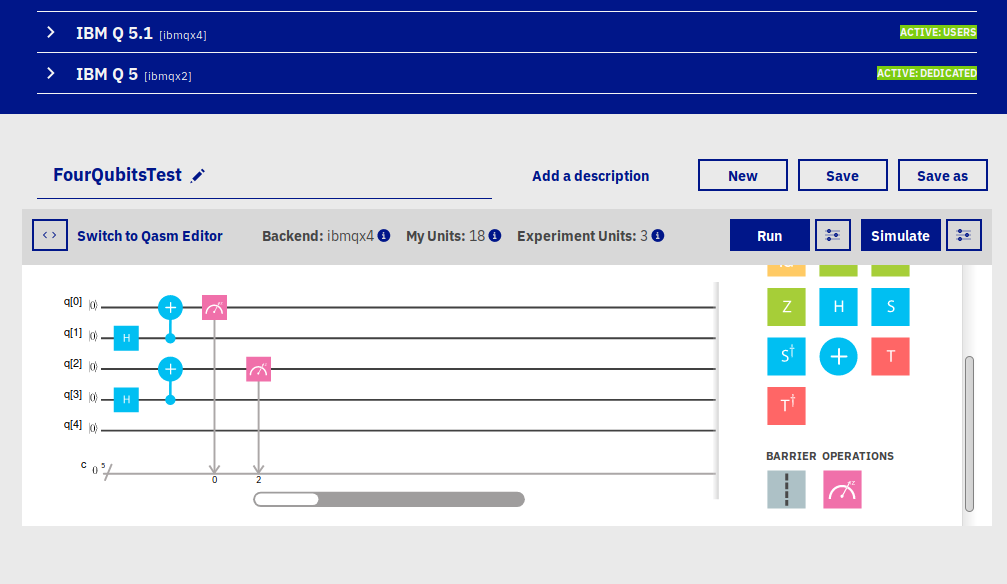
\includegraphics[height=0.65\textheight]{pics/ibm-q-experience-composer.png}
        \url{https://quantumexperience.ng.bluemix.net/qx/editor}
    \end{center}
\end{frame}

\begin{frame}{\insertsection}{\insertsubsection}
    \begin{center}
        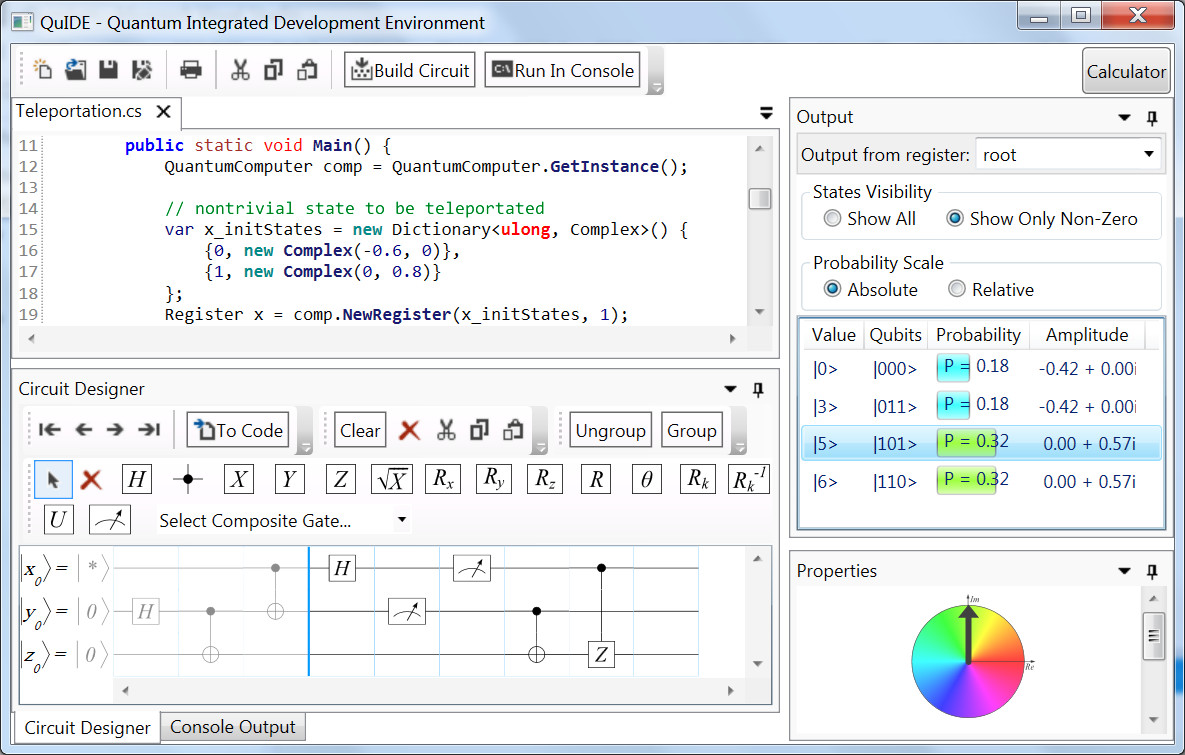
\includegraphics[height=0.7\textheight]{pics/QuIDE_GUI.jpg}
        \url{http://www.quide.eu/} and \url{https://bitbucket.org/quide/}
\end{center}      
\end{frame}

\begin{frame}{\insertsection}{\insertsubsection}
    \begin{itemize}
        \item<1-> Direct manipulation of quantum gates, measurement.
        \item<2-> Integration with text-based description of circuits: QASM 
        (IBM Q) or C\texttt{\#} (QuIDE).
        \item<3-> Useful for testing small circuits.
        \item<4-> Not so much for real algorithms.
        \item<5-> You have to live with connectivity limitations (IBM Q).
        \item<6-> But you can use a real quantum computer!
    \end{itemize}
\end{frame}   
    

%%%%%%%%%%%%%%%%%%%%%%%%%%%%%%%%%%%%%%%%%%%%%%%%%%%%%%%%%%%%%%%%%%%%%%%%%%%%%%%%
\subsection{Alternative approach: Manipulation of vectors and matrices}
%%%%%%%%%%%%%%%%%%%%%%%%%%%%%%%%%%%%%%%%%%%%%%%%%%%%%%%%%%%%%%%%%%%%%%%%%%%%%%%%

\begin{frame}{\insertsection}{\insertsubsection}
    You already know that
    \begin{itemize}
        \item<1-> quantum states are just vectors (at least we would like them 
        to 
        be)
        \item<2-> ...quantum gates are just matrices (at most $4\times 4$, and 
        don't mention the decoherence)...
        \item<3-> ...only the final step is somehow strange.
        \item<4->{\emph{Real Programmers do Quantum Computing in FORTRAN.}}
    \end{itemize}

\end{frame}

\begin{frame}{\insertsection}{\insertsubsection}
For example, in Julia... \\[12pt] \only<2->{Examples in 
Wolfram can be found in the GitHub repo}
\end{frame}

\begin{frame}{\insertsection}{\insertsubsection}
    \begin{itemize}
        \item<1-> Actually this is almost as good as it gets!
        \item<2-> Because...
        \begin{itemize}
            \item<3->  ...you already know the language.
            \item<4-> ...it is very easy to implement 
            classical control.
            \item<5-> ...it is relatively easy to take into account effects of 
            decoherence.
        \end{itemize}
        \item<6-> Missing: the memory management.
        \item<7-> And in most cases you don't need all the power/libraries/etc 
        coming with the host language.
    \end{itemize}
\end{frame}

%%%%%%%%%%%%%%%%%%%%%%%%%%%%%%%%%%%%%%%%%%%%%%%%%%%%%%%%%%%%%%%%%%%%%%%%%%%%%%%%
\subsection{Where to go next?}
%%%%%%%%%%%%%%%%%%%%%%%%%%%%%%%%%%%%%%%%%%%%%%%%%%%%%%%%%%%%%%%%%%%%%%%%%%%%%%%%
\begin{frame}{\insertsection}{\insertsubsection}
    \begin{itemize}
    \item<1-> IBM Q Experience: 
    {\small\url{https://quantumexperience.ng.bluemix.net/qx/editor}}
    \item<2-> Packages/matrix manipulation libraries:
    \begin{itemize}
        \item<3-> quantum-octave (Octave/Matlab): 
        {\small \url{https://github.com/ZKSI/quantum-octave}}
        \item<4-> QuTiP (Python library): {\small\url{http://qutip.org/}}
    \end{itemize}
    \item<5-> Many more at Quantiki 
    \url{https://quantiki.org/wiki/list-qc-simulators}
    \end{itemize}
\end{frame}

%%%%%%%%%%%%%%%%%%%%%%%%%%%%%%%%%%%%%%%%%%%%%%%%%%%%%%%%%%%%%%%%%%%%%%%%%%%%%%
\section{Programming QRAM}
%%%%%%%%%%%%%%%%%%%%%%%%%%%%%%%%%%%%%%%%%%%%%%%%%%%%%%%%%%%%%%%%%%%%%%%%%%%%%%

\begin{frame}
    \begin{center}
    {\color{iitis-orange} \LARGE \insertsection}
    \end{center}
\end{frame}


%%%%%%%%%%%%%%%%%%%%%%%%%%%%%%%%%%%%%%%%%%%%%%%%%%%%%%%%%%%%%%%%%%%%%%%%%%%%%%
\subsection{What is QRAM?}
%%%%%%%%%%%%%%%%%%%%%%%%%%%%%%%%%%%%%%%%%%%%%%%%%%%%%%%%%%%%%%%%%%%%%%%%%%%%%%
\begin{frame}{\insertsection}{\insertsubsection}
	\begin{center}
	QRAM $\equiv$ Quantum Random Access Machine\\[12pt]
    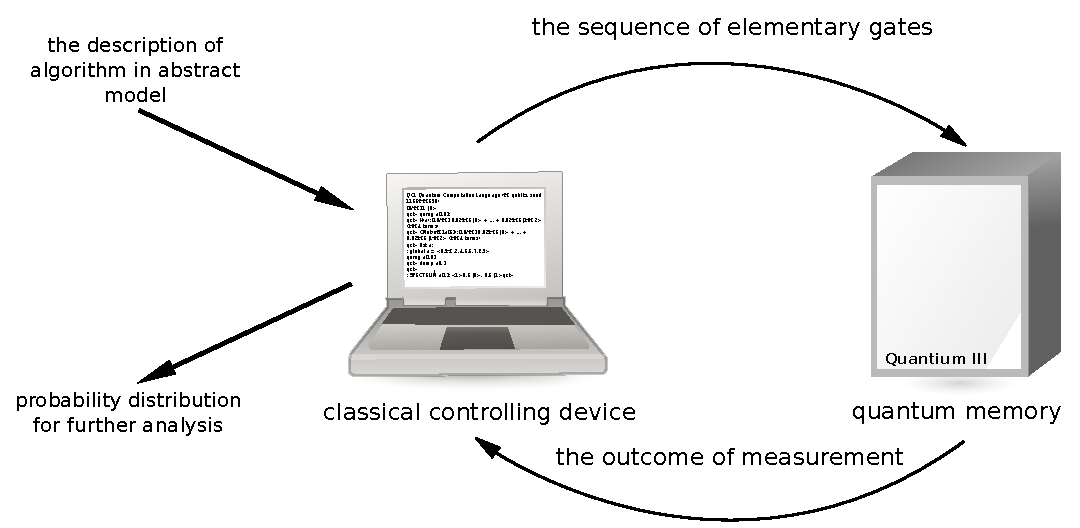
\includegraphics[width=\textwidth]{pics/qram}
\end{center}
\end{frame}

%%%%%%%%%%%%%%%%%%%%%%%%%%%%%%%%%%%%%%%%%%%%%%%%%%%%%%%%%%%%%%%%%%%%%%%%%%%%%%
\subsection{Advantages of QRAM}
%%%%%%%%%%%%%%%%%%%%%%%%%%%%%%%%%%%%%%%%%%%%%%%%%%%%%%%%%%%%%%%%%%%%%%%%%%%%%%
\begin{frame}{\insertsection}{\insertsubsection}
\begin{itemize}
	\item<1-> data abstraction \only<2->{$\equiv$ allocation of quantum memory}
	\item<3-> compound quantum operations \only<1-3>{\phantom{$\equiv$ 
	functions encapsulating sequence of quantum gates or quantum primitives}}%
    \only<4->{$\equiv$ functions encapsulating sequence of quantum gates or 
    quantum primitives}
	\item<5-> classical control of quantum operations
    \only<1-5>{\phantom{$\equiv$ loops, ifs etc. mixed with quantum code}}%
    \only<6->{$\equiv$ loops, ifs etc. mixed with quantum code}
\end{itemize}

\end{frame}

%%%%%%%%%%%%%%%%%%%%%%%%%%%%%%%%%%%%%%%%%%%%%%%%%%%%%%%%%%%%%%%%%%%%%%%%%%%%%%
\subsection{Software architecture}
%%%%%%%%%%%%%%%%%%%%%%%%%%%%%%%%%%%%%%%%%%%%%%%%%%%%%%%%%%%%%%%%%%%%%%%%%%%%%%
%%%%%%%%%%%%%%%%%%%%%%%%%%%%%%%%%%%%%%%%%%%%%%%%%%%%%%%%%%%%%%%%%%%%%%%%%%%%%%
\begin{frame}{\insertsection}{\insertsubsection}
    
\begin{center}
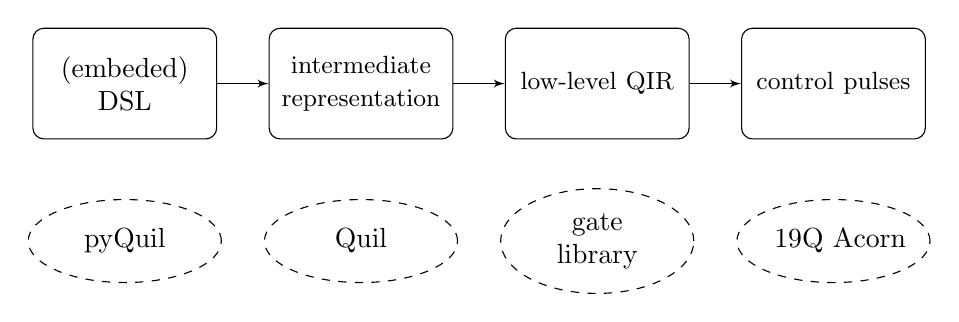
\begin{tikzpicture}[node distance = 3cm, auto]
\tikzstyle{block} = [rectangle, draw, text width=2.1cm, text centered, rounded 
corners, minimum height=4em]
\tikzstyle{example} = [draw, ellipse, node distance=2cm,  text width=1.5cm, 
dashed,
text centered, minimum  height=3em]
\tikzstyle{line} = [draw, -latex', thin]

\node [block] (edsl) {(embeded) DSL};
\node [example, below of=edsl] (edsl-ex) {pyQuil};

\node [block, right of=edsl] (qir) {\small intermediate representation};
\node [example, below of=qir] (qir-ex) {Quil};

\node [block, right of=qir] (qoptim) {\small low-level QIR};
\node [example, below of=qoptim] (qoptim-ex) {gate library};

\node [block, right of=qoptim] (qcontrol) {\small control pulses};
\node [example, below of=qcontrol] (qcontrol-ex) {19Q~Acorn};

\path [line] (edsl) -- (qir);
\path [line] (qir) -- (qoptim);
\path [line] (qoptim) -- (qcontrol);
\end{tikzpicture}
\end{center}
\end{frame}


%%%%%%%%%%%%%%%%%%%%%%%%%%%%%%%%%%%%%%%%%%%%%%%%%%%%%%%%%%%%%%%%%%%%%%%%%%%%%%
\subsection{Quantum middleware}
%%%%%%%%%%%%%%%%%%%%%%%%%%%%%%%%%%%%%%%%%%%%%%%%%%%%%%%%%%%%%%%%%%%%%%%%%%%%%%

\begin{frame}{\insertsection}{\insertsubsection}
	\begin{itemize}
		\item<1-> embedded domain specific language $\rightarrow$ 
		C/Python/Wolfram/Haskell
		with library of functions
		\item<2-> data abstraction $\rightarrow$ allocation of classical and quantum registers based on qu(b$|$d)its
		\item<3-> quantum functions $\rightarrow$ custom elementary gates defined by matrices or compound statements
		\item<4-> classical control of quantum memory $\rightarrow$ by using host language
	\end{itemize}
\end{frame}

%%%%%%%%%%%%%%%%%%%%%%%%%%%%%%%%%%%%%%%%%%%%%%%%%%%%%%%%%%%%%%%%%%%%%%%%%%%%%%
\subsection{...its advantages...}
%%%%%%%%%%%%%%%%%%%%%%%%%%%%%%%%%%%%%%%%%%%%%%%%%%%%%%%%%%%%%%%%%%%%%%%%%%%%%%
\begin{frame}{\insertsection}{\insertsubsection}
	\begin{itemize}
        \item<1-> easy to learn and use \only<article>{because you already know 
        the language}
		\item<2-> auto-magic quantum memory management \only<article>{because 
		qubits are just arrays}
        \item<3-> integration with classical machine
        \only<article>{obviously}
	\end{itemize}
\end{frame}

%%%%%%%%%%%%%%%%%%%%%%%%%%%%%%%%%%%%%%%%%%%%%%%%%%%%%%%%%%%%%%%%%%%%%%%%%%%%%%
\subsection{...and its disadvantages}
%%%%%%%%%%%%%%%%%%%%%%%%%%%%%%%%%%%%%%%%%%%%%%%%%%%%%%%%%%%%%%%%%%%%%%%%%%%%%%
\begin{frame}{\insertsection}{\insertsubsection}
    \begin{itemize}
        \item<1-> very similar to low-level code \only<article<>{(but library 
        of gates can be build)}
        \item<2-> lack of expressibility \only<article>{$\equiv$ you operate on 
        basic ingredients only}
    \end{itemize}
\end{frame}

%%%%%%%%%%%%%%%%%%%%%%%%%%%%%%%%%%%%%%%%%%%%%%%%%%%%%%%%%%%%%%%%%%%%%%%%%%%%%%
\subsection{Example 1: ProjectQ}
%%%%%%%%%%%%%%%%%%%%%%%%%%%%%%%%%%%%%%%%%%%%%%%%%%%%%%%%%%%%%%%%%%%%%%%%%%%%%%

\begin{frame}{\insertsection}{\insertsubsection}
	\begin{itemize}
        \item Python library developed by ETH (\url{https://projectq.ch/})
        \item offers various targets
        \begin{itemize}
            \item hardware (IBM Q Experience) 
            \only<article>{(\verb|use_hardware=False|)}
            \item resource counter (???)
            \item graphical circuit representation
        \end{itemize}
    \end{itemize}
\end{frame}


%%%%%%%%%%%%%%%%%%%%%%%%%%%%%%%%%%%%%%%%%%%%%%%%%%%%%%%%%%%%%%%%%%%%%%%%%%%%%%
\begin{frame}{\insertsection}{\insertsubsection}
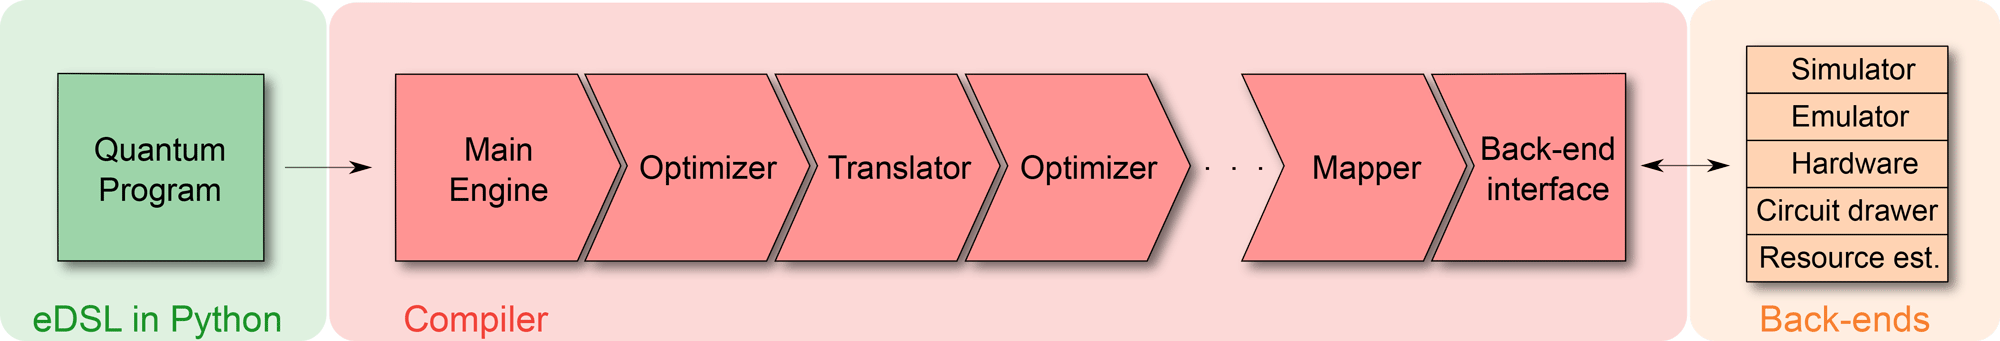
\includegraphics[width=\textwidth]{pics/projectq-compiler-overview.png}\\

\end{frame}

%%%%%%%%%%%%%%%%%%%%%%%%%%%%%%%%%%%%%%%%%%%%%%%%%%%%%%%%%%%%%%%%%%%%%%%%%%%%%%
\begin{frame}{\insertsection}{\insertsubsection}
    Nice features
    \begin{itemize}
        \item Natural (for physicist) syntax for executing quantum gates.
        \item Meta instructions for quantum-controlled quantum operations and 
        support for reverse call
        \only<article>{(very easy to construct controlled operations)}
    \end{itemize}
\end{frame}

%%%%%%%%%%%%%%%%%%%%%%%%%%%%%%%%%%%%%%%%%%%%%%%%%%%%%%%%%%%%%%%%%%%%%%%%%%%%%%
\begin{frame}{\insertsection}{\insertsubsection}
Some examples...
\end{frame}

%%%%%%%%%%%%%%%%%%%%%%%%%%%%%%%%%%%%%%%%%%%%%%%%%%%%%%%%%%%%%%%%%%%%%%%%%%%%%%
\begin{frame}{\insertsection}{\insertsubsection}
    \begin{block}{Metainstruction \texttt{Control}}
        Execution of the code is based on the state of quantum register.
    \end{block}

    \begin{center}
     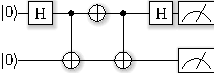
\includegraphics[scale=1.5]{pics/meta_control_circ.pdf}
    \end{center}
\end{frame}

%%%%%%%%%%%%%%%%%%%%%%%%%%%%%%%%%%%%%%%%%%%%%%%%%%%%%%%%%%%%%%%%%%%%%%%%%%%%%%
\begin{frame}{\insertsection}{\insertsubsection}
    \begin{block}{Metainstruction \texttt{Dagger}}
        Reverse execution of the quantum code.
    \end{block}
    
    \begin{center}
        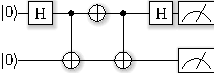
\includegraphics[scale=1.5]{pics/meta_dagger_circ.pdf}
    \end{center}
\end{frame}

%%%%%%%%%%%%%%%%%%%%%%%%%%%%%%%%%%%%%%%%%%%%%%%%%%%%%%%%%%%%%%%%%%%%%%%%%%%%%%
\subsection{Example 2: Rigetti Forest and pyQuil}
%%%%%%%%%%%%%%%%%%%%%%%%%%%%%%%%%%%%%%%%%%%%%%%%%%%%%%%%%%%%%%%%%%%%%%%%%%%%%%

\begin{frame}{\insertsection}{\insertsubsection}
	\begin{itemize}
        \item<1-> Quil $\equiv$ quantum assembly language.
        \item<2-> pyQuil $\equiv$ Python library for manipulating quantum 
        programmes in Quill.
        \item<3-> Access to Rigetti 19Q-Acorn quantum computer!
        \item<4-> More during the third day: Adam Szady, Quantum programming 
        with (Py)Quil.
    \end{itemize}
\end{frame}


%%%%%%%%%%%%%%%%%%%%%%%%%%%%%%%%%%%%%%%%%%%%%%%%%%%%%%%%%%%%%%%%%%%%%%%%%%%%%%
\section{High-level programming}
%%%%%%%%%%%%%%%%%%%%%%%%%%%%%%%%%%%%%%%%%%%%%%%%%%%%%%%%%%%%%%%%%%%%%%%%%%%%%%


%%%%%%%%%%%%%%%%%%%%%%%%%%%%%%%%%%%%%%%%%%%%%%%%%%%%%%%%%%%%%%%%%%%%%%%%%%%%%%
\subsection{Domain specific languages}
%%%%%%%%%%%%%%%%%%%%%%%%%%%%%%%%%%%%%%%%%%%%%%%%%%%%%%%%%%%%%%%%%%%%%%%%%%%%%%

\begin{frame}{\insertsection}{\insertsubsection}

\begin{block}{Level 2}
Domain specific language with data and function abstraction.
\end{block}

\begin{itemize}
    \item QCL (\url{http://tph.tuwien.ac.at/~oemer/qcl.html})
    \item LanQ (\url{http://lanq.sourceforge.net/})
    \item QPL anc cQPL (\url{https://arxiv.org/abs/quant-ph/0511145})
    \item Scaffold (\url{https://github.com/epiqc/ScaffCC})
\end{itemize}
\end{frame}


%%%%%%%%%%%%%%%%%%%%%%%%%%%%%%%%%%%%%%%%%%%%%%%%%%%%%%%%%%%%%%%%%%%%%%%%%%%%%%
\subsection{Example 1: QCL -- focus on quantum computing}
%%%%%%%%%%%%%%%%%%%%%%%%%%%%%%%%%%%%%%%%%%%%%%%%%%%%%%%%%%%%%%%%%%%%%%%%%%%%%%

%%%%%%%%%%%%%%%%%%%%%%%%%%%%%%%%%%%%%%%%%%%%%%%%%%%%%%%%%%%%%%%%%%%%%%%%%%%%%%
\begin{frame}{\insertsection}{\insertsubsection}
	\begin{itemize}
		\item<1-> First release in 1998, last in 2014 
		(\url{http://tph.tuwien.ac.at/~oemer/qcl.html}).
		\item<2-> Architecture independent programming language for quantum 
		computers.

	\end{itemize}
	
\end{frame}

%%%%%%%%%%%%%%%%%%%%%%%%%%%%%%%%%%%%%%%%%%%%%%%%%%%%%%%%%%%%%%%%%%%%%%%%%%%%%%
\begin{frame}{\insertsection}{\insertsubsection}
    Features
    \begin{itemize}
        \item<1-> Syntax for reversibility (uncomputing).
        \item<2-> Different types of quantum memory for better optimization.
        \item<3-> Quantum conditions --- quantum-controlled execution 
        (generalization of controlled 
        gates).
        \item<4-> Various types of compound statements (related with memory 
        management): quantum operators, quantum functions, procedures.

    \end{itemize}
\end{frame}

%%%%%%%%%%%%%%%%%%%%%%%%%%%%%%%%%%%%%%%%%%%%%%%%%%%%%%%%%%%%%%%%%%%%%%%%%%%%%%
\begin{frame}{\insertsection}{\insertsubsection}
    Advanced quantum memory management using types:
    \begin{itemize}
        \item<1-> \texttt{qureg} ---  basic type for quantum registers,
        \item<2-> \texttt{quconst} --- cannot be modified,
        \item<3-> \texttt{quvoid} --- has to be empty before the call,
        \item<4-> \texttt{quscratch} --- has to be empty before and after the 
        call.
    \end{itemize}
\end{frame}


\begin{frame}{\insertsection}{\insertsubsection}
    Types of quantum functions:
    \begin{itemize}
        \item<1-> \texttt{procedure} ---  classically controlled quantum 
        computation,
        \item<2-> \texttt{qufunct} --- used to implement irreversible functions,
        \item<3-> \texttt{operator} --- compound quantum operation.
    \end{itemize}
\end{frame}

%%%%%%%%%%%%%%%%%%%%%%%%%%%%%%%%%%%%%%%%%%%%%%%%%%%%%%%%%%%%%%%%%%%%%%%%%%%%%%
\begin{frame}{\insertsection}{\insertsubsection}
Some examples...
\end{frame}

%%%%%%%%%%%%%%%%%%%%%%%%%%%%%%%%%%%%%%%%%%%%%%%%%%%%%%%%%%%%%%%%%%%%%%%%%%%%%%
\subsection{Example 2: cQPL -- focus on quantum communication}
%%%%%%%%%%%%%%%%%%%%%%%%%%%%%%%%%%%%%%%%%%%%%%%%%%%%%%%%%%%%%%%%%%%%%%%%%%%%%%

%%%%%%%%%%%%%%%%%%%%%%%%%%%%%%%%%%%%%%%%%%%%%%%%%%%%%%%%%%%%%%%%%%%%%%%%%%%%%%
\begin{frame}{\insertsection}{\insertsubsection}
    
    \begin{itemize}
        \item<1-> QPL (formal specification) and cQPL (implementation of QPL, 
        \url{https://arxiv.org/abs/quant-ph/0511145})
        \item<2-> Functional paradigm.
        \item<3-> No publicly available implementation.
        \item<4-> Syntax for creating quantum communication channels by sharing 
        (entangled) qubits.
    \end{itemize}
\end{frame}

%%%%%%%%%%%%%%%%%%%%%%%%%%%%%%%%%%%%%%%%%%%%%%%%%%%%%%%%%%%%%%%%%%%%%%%%%%%%%%
\section{What next?}
%%%%%%%%%%%%%%%%%%%%%%%%%%%%%%%%%%%%%%%%%%%%%%%%%%%%%%%%%%%%%%%%%%%%%%%%%%%%%%

%%%%%%%%%%%%%%%%%%%%%%%%%%%%%%%%%%%%%%%%%%%%%%%%%%%%%%%%%%%%%%%%%%%%%%%%%%%%%%
\begin{frame}{\insertsection}
	\begin{itemize}
		\item \textbf{IF} D-Wave \textbf{GOTO} Andy Mason and Sheir Yarkoni, 
		Tutorial on 
		programming the D-Wave system
		\item \textbf{IF} IBM \textbf{GOTO} Ram Du\v{s}i\'c Hren, IBM Q 
		Experience: Hands-on workshop
		\item \textbf{IF} Rigetti \textbf{GOTO} Adam Szady, Quantum programming 
		with (Py)Quil
	\end{itemize}
\end{frame}

%%%%%%%%%%%%%%%%%%%%%%%%%%%%%%%%%%%%%%%%%%%%%%%%%%%%%%%%%%%%%%%%%%%%%%%%%%%%%%
\section{Q?}
%%%%%%%%%%%%%%%%%%%%%%%%%%%%%%%%%%%%%%%%%%%%%%%%%%%%%%%%%%%%%%%%%%%%%%%%%%%%%%
%%%%%%%%%%%%%%%%%%%%%%%%%%%%%%%%%%%%%%%%%%%%%%%%%%%%%%%%%%%%%%%%%%%%%%%%%%%%%%
\begin{frame}{\insertsection}
    \begin{center}
        \Huge {\color{iitis-orange} \insertsection}\\[12pt]
%        \LARGE Thank you.\\[12pt]
        \large \url{https://github.com/jmiszczak/qprog-tutorial}
    \end{center}
\end{frame}

\end{document}
